\documentclass[14pt,a4paper]{extreport}

% Подключение пакетов
% Пакеты для работы с русским языком
\usepackage[utf8]{inputenc}
\usepackage[T2A]{fontenc}
\usepackage[english,russian]{babel}

% Пакеты для форматирования
\usepackage{geometry}
\usepackage{setspace}
\usepackage{indentfirst}
\usepackage{titlesec}
\usepackage{tocloft}

% Пакеты для математики
\usepackage{amsmath}
\usepackage{amsfonts}
\usepackage{amssymb}
\usepackage{mathtools}
% \usepackage{calc} % убираем calc из-за конфликта с кириллицей

% Пакеты для графики
\usepackage{graphicx}
\usepackage{float}
\usepackage{subcaption}
\usepackage{wrapfig}

% Пакеты для таблиц
\usepackage{array}
\usepackage{longtable}
\usepackage{booktabs}
\usepackage{tabularx}

% Пакеты для библиографии
\usepackage[style=gost-numeric,sorting=none,backend=biber,defernumbers=true]{biblatex}

% Пакеты для ссылок
\usepackage{hyperref}
\usepackage{url}
\usepackage{cleveref}

% Пакеты для кода
\usepackage{listings}
\usepackage{xcolor}

% Пакеты для специальных символов
\usepackage{textcomp}
\usepackage{gensymb}

% Пакеты для многострочных формул
% \usepackage{multline} % пакет не найден в BasicTeX

% Пакеты для алгоритмов
\usepackage{algorithm}
\usepackage{algorithmic}

% Пакеты для приложений
\usepackage{appendix}


% Настройки документа
% Настройки страницы по ГОСТ Р 7.0.11-2011 и ГОСТ 7.32-2017
\geometry{
    left=30mm,
    right=15mm,
    top=20mm,
    bottom=20mm
}

% Межстрочный интервал 1.5 по ГОСТу
\onehalfspacing

% Отступ первой строки абзаца 1.25 см по ГОСТу
\setlength{\parindent}{1.25cm}

% Настройки шрифтов по ГОСТу для pdfLaTeX
\usepackage{times}

% Настройки заголовков по ГОСТу 7.32-2017
\titleformat{\chapter}[display]
{\normalfont\bfseries\centering}
{\chaptertitlename\ \thechapter}{20pt}{\Large}

\titleformat{\section}
{\normalfont\bfseries}
{\thesection}{1em}{}

\titleformat{\subsection}
{\normalfont\bfseries}
{\thesubsection}{1em}{}

% Настройки оглавления по ГОСТу 7.32-2017
\renewcommand{\cftchapleader}{\cftdotfill{\cftdotsep}}
\renewcommand{\cftsecleader}{\cftdotfill{\cftdotsep}}
\renewcommand{\cftsubsecleader}{\cftdotfill{\cftdotsep}}

% Настройки отступов в оглавлении по ГОСТ 7.32-2017
\renewcommand{\cftchapindent}{0pt}  % Главы без отступа
\renewcommand{\cftsecindent}{2em}   % Разделы с отступом 2 знака
\renewcommand{\cftsubsecindent}{4em} % Подразделы с отступом 4 знака

% Настройки шрифтов в оглавлении
\renewcommand{\cftchapfont}{\bfseries}
\renewcommand{\cftsecfont}{\normalfont}
\renewcommand{\cftsubsecfont}{\normalfont}

% Настройки отступов между элементами
\setlength{\cftbeforechapskip}{0pt}
\setlength{\cftbeforesecskip}{0pt}
\setlength{\cftbeforesubsecskip}{0pt}

% Настройки библиографии
\addbibresource{bibliography/references.bib}

% Настройки стиля библиографии по ГОСТ 7.32-2017
\DeclareFieldFormat{labelnumberwidth}{#1.}
\setlength{\biblabelsep}{0.5em}
\renewcommand*{\bibfont}{\small}
\setlength{\bibhang}{1.25cm} % абзацный отступ по ГОСТу

% Настройки гиперссылок
\hypersetup{
    colorlinks=true,
    linkcolor=black,
    filecolor=magenta,      
    urlcolor=blue,
    citecolor=black,
    bookmarksnumbered=true,
    bookmarksopen=true,
    pdfstartview=FitH
}

% Настройки листингов кода
\lstset{
    basicstyle=\small\ttfamily,
    breaklines=true,
    frame=single,
    numbers=left,
    numberstyle=\tiny,
    stepnumber=1,
    numbersep=5pt,
    showstringspaces=false,
    showtabs=false,
    tabsize=2,
    captionpos=b,
    commentstyle=\color{gray},
    keywordstyle=\color{blue},
    stringstyle=\color{red}
}

% Настройки нумерации по ГОСТу 7.32-2017
\renewcommand{\thefigure}{\arabic{figure}}
\renewcommand{\thetable}{\arabic{table}}
\renewcommand{\theequation}{\arabic{equation}}

% Настройки подписей к рисункам и таблицам по ГОСТ 7.32-2017
\captionsetup[figure]{
    font=small,
    justification=centering,
    singlelinecheck=false,
    skip=0pt,  % межстрочный интервал 1.0 (обычный)
    belowskip=0pt,
    aboveskip=0pt,
    hypcap=false  % запрет переноса слов в подписях к рисункам
}

\captionsetup[table]{
    font=small,
    justification=raggedright,
    singlelinecheck=false,
    skip=0pt,
    belowskip=0pt,
    aboveskip=0pt,
    hypcap=false  % запрет переноса слов в подписях к таблицам
}

% Переопределяем формат подписей для соответствия ГОСТу
\renewcommand{\figurename}{Рисунок}
\renewcommand{\tablename}{Таблица}

% Настройка формата подписи к рисунку по ГОСТ 7.32-2017
\DeclareCaptionFormat{gostfigure}{#1#2 — #3}
\captionsetup[figure]{format=gostfigure}

% Настройка формата подписи к таблице по ГОСТ 7.32-2017
\DeclareCaptionFormat{gosttable}{#1#2 — #3}
\captionsetup[table]{format=gosttable}

% Настройка переноса таблиц с заголовком "Продолжение таблицы X"
\usepackage{longtable}
\usepackage{ltxtable}

% Команда для создания продолжения таблицы
\newcommand{\tablecontinuation}[1]{%
    \multicolumn{1}{c}{\textbf{Продолжение таблицы #1}}%
}

% Настройка переноса листингов кода
\usepackage{fancyvrb}
\usepackage{listings}

% Настройки для переноса листингов
\lstset{
    breaklines=true,
    breakatwhitespace=true,
    breakautoindent=true,
    postbreak=\mbox{\textcolor{red}{$\hookrightarrow$}\space},
    frame=single,
    numbers=left,
    numberstyle=\tiny,
    stepnumber=1,
    numbersep=5pt,
    showstringspaces=false,
    showtabs=false,
    tabsize=2,
    basicstyle=\ttfamily\small,
    keywordstyle=\color{blue}\bfseries,
    commentstyle=\color{green!60!black},
    stringstyle=\color{red},
    extendedchars=true,
    inputencoding=utf8,
    literate={а}{{\cyra}}1 {б}{{\cyrb}}1 {в}{{\cyrv}}1 {г}{{\cyrg}}1 {д}{{\cyrd}}1 {е}{{\cyre}}1 {ё}{{\cyryo}}1 {ж}{{\cyrzh}}1 {з}{{\cyrz}}1 {и}{{\cyri}}1 {й}{{\cyrishrt}}1 {к}{{\cyrk}}1 {л}{{\cyrl}}1 {м}{{\cyrm}}1 {н}{{\cyrn}}1 {о}{{\cyro}}1 {п}{{\cyrp}}1 {р}{{\cyrr}}1 {с}{{\cyrs}}1 {т}{{\cyrt}}1 {у}{{\cyru}}1 {ф}{{\cyrf}}1 {х}{{\cyrh}}1 {ц}{{\cyrc}}1 {ч}{{\cyrch}}1 {ш}{{\cyrsh}}1 {щ}{{\cyrshch}}1 {ъ}{{\cyrhrdsn}}1 {ы}{{\cyry}}1 {ь}{{\cyrsftsn}}1 {э}{{\cyrerev}}1 {ю}{{\cyryu}}1 {я}{{\cyrya}}1
}

% Настройка для автоматического переноса длинных листингов
\usepackage{fancyvrb}
\DefineVerbatimEnvironment{Code}{Verbatim}{
    fontsize=\small,
    frame=single,
    numbers=left,
    numberstyle=\tiny,
    stepnumber=1,
    numbersep=5pt,
    breaklines=true,
    breakanywhere=true
}

% Настройка для автоматического переноса листингов с продолжением
\lstdefinestyle{breakable}{
    breaklines=true,
    breakatwhitespace=true,
    breakautoindent=true,
    postbreak=\mbox{\textcolor{red}{$\hookrightarrow$}\space},
    frame=single,
    numbers=left,
    numberstyle=\tiny,
    stepnumber=1,
    numbersep=5pt,
    showstringspaces=false,
    showtabs=false,
    tabsize=2,
    basicstyle=\ttfamily\small,
    keywordstyle=\color{blue}\bfseries,
    commentstyle=\color{green!60!black},
    stringstyle=\color{red},
    extendedchars=true,
    inputencoding=utf8,
    literate={а}{{\cyra}}1 {б}{{\cyrb}}1 {в}{{\cyrv}}1 {г}{{\cyrg}}1 {д}{{\cyrd}}1 {е}{{\cyre}}1 {ё}{{\cyryo}}1 {ж}{{\cyrzh}}1 {з}{{\cyrz}}1 {и}{{\cyri}}1 {й}{{\cyrishrt}}1 {к}{{\cyrk}}1 {л}{{\cyrl}}1 {м}{{\cyrm}}1 {н}{{\cyrn}}1 {о}{{\cyro}}1 {п}{{\cyrp}}1 {р}{{\cyrr}}1 {с}{{\cyrs}}1 {т}{{\cyrt}}1 {у}{{\cyru}}1 {ф}{{\cyrf}}1 {х}{{\cyrh}}1 {ц}{{\cyrc}}1 {ч}{{\cyrch}}1 {ш}{{\cyrsh}}1 {щ}{{\cyrshch}}1 {ъ}{{\cyrhrdsn}}1 {ы}{{\cyry}}1 {ь}{{\cyrsftsn}}1 {э}{{\cyrerev}}1 {ю}{{\cyryu}}1 {я}{{\cyrya}}1
}

% Настройка для переноса длинных листингов
\usepackage{fancyvrb}
\DefineVerbatimEnvironment{Code}{Verbatim}{
    fontsize=\small,
    frame=single,
    numbers=left,
    numberstyle=\tiny,
    stepnumber=1,
    numbersep=5pt,
    breaklines=true,
    breakanywhere=true
}

% Команда для создания продолжения листинга
\newcommand{\listingcontinuation}[1]{%
    \textbf{Продолжение листинга #1}%
}

% Настройки примечаний согласно ГОСТ 7.32-2017
\newcommand{\note}[1]{%
    \par\noindent\textbf{Примечание} — #1%
}

\newcommand{\notes}[1]{%
    \par\noindent\textbf{Примечания:}%
    \begin{enumerate}
        #1
    \end{enumerate}%
}

% Настройка межстрочного интервала для многострочных подписей
\captionsetup[table]{format=gosttable,skip=6pt}  % межстрочный интервал 1.0

% Настройки списков рисунков и таблиц
\renewcommand{\listfigurename}{СПИСОК ИЛЛЮСТРАЦИЙ}
\renewcommand{\listtablename}{СПИСОК ТАБЛИЦ}

% Настройки приложений
\renewcommand{\appendixname}{Приложение}
\renewcommand{\appendixpagename}{Приложения}

% ===== АВТОМАТИЧЕСКИЕ ПРАВИЛА ГОСТ =====

% Автоматические переносы слов по ГОСТу
\usepackage[english,russian]{babel}
\babelprovide[import]{russian}
\babelprovide[import]{english}

% Автоматические отступы для списков по ГОСТу
\setlength{\leftmargini}{2.5em}  % отступ для enumerate
\setlength{\leftmarginii}{2em}   % отступ для вложенных списков
\setlength{\leftmarginiii}{1.5em}
\setlength{\leftmarginiv}{1em}

% Автоматическое форматирование списков
\renewcommand{\labelenumi}{\arabic{enumi})}
\renewcommand{\labelenumii}{\arabic{enumi}.\arabic{enumii})}
\renewcommand{\labelenumiii}{\arabic{enumi}.\arabic{enumii}.\arabic{enumiii})}
\renewcommand{\labelenumiv}{\arabic{enumi}.\arabic{enumii}.\arabic{enumiii}.\arabic{enumiv})}

% Автоматические отступы для itemize
\renewcommand{\labelitemi}{---}
\renewcommand{\labelitemii}{--}
\renewcommand{\labelitemiii}{-}
\renewcommand{\labelitemiv}{.}

% Автоматическое форматирование формул по ГОСТу
\renewcommand{\theequation}{\arabic{equation}}
\setlength{\abovedisplayskip}{6pt}
\setlength{\belowdisplayskip}{6pt}
\setlength{\abovedisplayshortskip}{0pt}
\setlength{\belowdisplayshortskip}{0pt}

% Автоматические правила для ссылок
\renewcommand{\autoref}[1]{\textbf{\ref{#1}}}
\renewcommand{\nameref}[1]{\textbf{\ref{#1}}}

% Автоматические правила для абзацев
\setlength{\parskip}{0pt}  % без отступов между абзацами
\setlength{\parindent}{1.25cm}  % отступ первой строки по ГОСТу

% Автоматические правила для переноса страниц
\widowpenalty=10000
\clubpenalty=10000
\raggedbottom

% Автоматические правила для переноса слов в тексте
\hyphenpenalty=50
\exhyphenpenalty=50
\doublehyphendemerits=10000
\finalhyphendemerits=5000

% Автоматические правила для таблиц
\setlength{\tabcolsep}{6pt}
\setlength{\arrayrulewidth}{0.4pt}
\renewcommand{\arraystretch}{1.2}

% Автоматические правила для рисунков
\setlength{\floatsep}{12pt}
\setlength{\textfloatsep}{12pt}
\setlength{\intextsep}{12pt}

% Автоматические правила для примечаний
\newcommand{\autonote}[1]{%
    \par\noindent\textbf{Примечание} — #1%
}

% Автоматические правила для списков литературы
\renewcommand{\bibname}{СПИСОК ИСПОЛЬЗОВАННЫХ ИСТОЧНИКОВ}

% Автоматические правила для оглавления
\renewcommand{\contentsname}{ОГЛАВЛЕНИЕ}

% Автоматические правила для реферата
\renewcommand{\abstractname}{РЕФЕРАТ}

% Автоматические правила для заключения
\providecommand{\conclusionname}{ЗАКЛЮЧЕНИЕ}

% Автоматические правила для введения
\providecommand{\introductionname}{ВВЕДЕНИЕ}

% ===== АВТОМАТИЧЕСКИЕ КОМАНДЫ ДЛЯ УПРОЩЕНИЯ НАПИСАНИЯ =====
% Эти команды применяют правила ГОСТ автоматически

% Автоматическое создание рисунка с правильным форматированием
\newcommand{\autofigure}[4]{%
    \begin{figure}[H]%
        \centering%
        \includegraphics[width=#2]{#1}%
        \caption{#3}%
        \label{#4}%
    \end{figure}%
}

% Автоматическое создание таблицы с правильным форматированием
\newcommand{\autotable}[3]{%
    \begin{table}[H]%
        \centering%
        \caption{#2}%
        \label{#3}%
        #1%
    \end{table}%
}

% Автоматическое создание формулы с правильным форматированием
\newcommand{\autoformula}[2]{%
    \begin{equation}%
        #1%
        \label{#2}%
    \end{equation}%
}

% Автоматическое создание списка с правильным форматированием
\newcommand{\autolist}[1]{%
    \begin{enumerate}%
        #1%
    \end{enumerate}%
}

% Автоматическое создание маркированного списка
\newcommand{\autobulletlist}[1]{%
    \begin{itemize}%
        #1%
    \end{itemize}%
}

% Автоматическое создание ссылки с правильным форматированием
\providecommand{\autoref}[1]{%
    \textbf{\ref{#1}}%
}

% Автоматическое создание ссылки на рисунок
\newcommand{\autofigref}[1]{%
    \textbf{рисунок \ref{#1}}%
}

% Автоматическое создание ссылки на таблицу
\newcommand{\autotableref}[1]{%
    \textbf{таблица \ref{#1}}%
}

% Автоматическое создание ссылки на формулу
\newcommand{\autoformularef}[1]{%
    \textbf{формула \ref{#1}}%
}

% Автоматическое создание примечания
\providecommand{\autonote}[1]{%
    \par\noindent\textbf{Примечание} — #1%
}

% Автоматическое создание нескольких примечаний
\newcommand{\autonotes}[1]{%
    \par\noindent\textbf{Примечания:}%
    \begin{enumerate}%
        #1%
    \end{enumerate}%
}

% Автоматическое создание абзаца с правильным отступом
\newcommand{\autopar}[1]{%
    \par\noindent#1%
}

% Автоматическое создание заголовка раздела
\newcommand{\autosection}[1]{%
    \section{#1}%
}

% Автоматическое создание заголовка подраздела
\newcommand{\autosubsection}[1]{%
    \subsection{#1}%
}

% Автоматическое создание заголовка главы
\newcommand{\autochapter}[1]{%
    \chapter{#1}%
}


% Начало документа
\begin{document}

% Титульный лист
\begin{titlepage}
    \begin{center}
        \vspace*{1cm}
        
        \textbf{МИНИСТЕРСТВО НАУКИ И ВЫСШЕГО ОБРАЗОВАНИЯ РОССИЙСКОЙ ФЕДЕРАЦИИ}\\
        \textbf{Федеральное государственное автономное образовательное учреждение высшего образования}\\
        \textbf{«НАЗВАНИЕ УНИВЕРСИТЕТА»}
        
        \vspace{1cm}
        
        \textbf{НАЗВАНИЕ ИНСТИТУТА/ФАКУЛЬТЕТА}\\
        \textbf{Кафедра НАЗВАНИЕ КАФЕДРЫ}
        
        \vspace{2cm}
        
        \textbf{ВЫПУСКНАЯ КВАЛИФИКАЦИОННАЯ РАБОТА}\\
        \textbf{на тему:}\\
        \textbf{«НАЗВАНИЕ ТЕМЫ ДИССЕРТАЦИИ»}
        
        \vspace{1cm}
        
        \textbf{Направление подготовки:} КОД И НАЗВАНИЕ НАПРАВЛЕНИЯ\\
        \textbf{Профиль:} НАЗВАНИЕ ПРОФИЛЯ
        
        \vspace{2cm}
        
        \textbf{Выполнил:}\\
        студент группы НОМЕР ГРУППЫ\\
        ФАМИЛИЯ И.О.
        
        \vspace{0.5cm}
        
        \textbf{Руководитель:}\\
        УЧЕНАЯ СТЕПЕНЬ, ЗВАНИЕ\\
        ФАМИЛИЯ И.О.
        
        \vspace{0.5cm}
        
        \textbf{Консультант:}\\
        УЧЕНАЯ СТЕПЕНЬ, ЗВАНИЕ\\
        ФАМИЛИЯ И.О.
        
        \vfill
        
        \textbf{ГОРОД}\\
        \textbf{ГОД}
        
    \end{center}
\end{titlepage}


% Реферат (обязательно по ГОСТ 7.32-2017)
% Реферат по ГОСТ 7.32-2017
\begin{center}
    \textbf{РЕФЕРАТ}
\end{center}

\vspace{1cm}

\textbf{Объем работы:} [X] страниц, [Y] рисунков, [Z] таблиц, [N] источников.

\textbf{Ключевые слова:} [КЛЮЧЕВОЕ СЛОВО 1], [КЛЮЧЕВОЕ СЛОВО 2], [КЛЮЧЕВОЕ СЛОВО 3], [КЛЮЧЕВОЕ СЛОВО 4], [КЛЮЧЕВОЕ СЛОВО 5].

\vspace{1cm}

[Здесь должен быть краткий реферат работы объемом 1-2 страницы, включающий:
- Цель и задачи исследования
- Объект и предмет исследования  
- Методы исследования
- Основные результаты и их новизну
- Практическую значимость
- Степень внедрения и эффективность
- Рекомендации по использованию результатов]

\vspace{1cm}

\textbf{Аннотация на английском языке:}

\textbf{Abstract}

\textbf{Volume:} [X] pages, [Y] figures, [Z] tables, [N] sources.

\textbf{Keywords:} [KEYWORD 1], [KEYWORD 2], [KEYWORD 3], [KEYWORD 4], [KEYWORD 5].

\vspace{1cm}

[English abstract here - translation of the Russian abstract]

\newpage


% Оглавление по ГОСТу
\tableofcontents
\newpage

% Введение
\chapter{Введение}

\section{Актуальность темы исследования}

Текст актуальности исследования. Здесь необходимо обосновать важность выбранной темы, показать её значимость для науки и практики.

\section{Степень разработанности проблемы}

Анализ существующих исследований по теме. Обзор работ отечественных и зарубежных авторов.

\section{Цель и задачи исследования}

\subsection{Цель исследования}

Сформулировать основную цель работы.

\subsection{Задачи исследования}

\begin{enumerate}
    \item Первая задача;
    \item Вторая задача;
    \item Третья задача;
    \item И так далее.
\end{enumerate}

\section{Объект и предмет исследования}

\subsection{Объект исследования}

Описание объекта исследования.

\subsection{Предмет исследования}

Описание предмета исследования.

\section{Методы исследования}

Перечисление методов, используемых в работе.

\section{Научная новизна}

Описание научной новизны исследования.

\section{Практическая значимость}

Описание практической значимости результатов работы.

\section{Структура работы}

Краткое описание структуры диссертации с указанием количества страниц в каждой главе.

\section{Апробация результатов}

Информация о публикациях, выступлениях на конференциях и других формах апробации результатов.


% Основная часть
\chapter{ТЕОРЕТИЧЕСКИЕ ОСНОВЫ ИССЛЕДОВАНИЯ}

\section{Основные понятия и определения}

Здесь приводятся основные понятия, используемые в работе, их определения и взаимосвязи.

\subsection{Понятие 1}

Определение и характеристика первого ключевого понятия.

\subsection{Понятие 2}

Определение и характеристика второго ключевого понятия.

\section{Анализ существующих подходов}

Обзор и анализ различных подходов к решению исследуемой проблемы.

\subsection{Подход 1}

Описание первого подхода, его достоинства и недостатки.

\subsection{Подход 2}

Описание второго подхода, его достоинства и недостатки.

\section{Методологические основы}

Описание методологических основ исследования.

\section{Выводы по главе}

Краткие выводы по теоретической части работы.

\chapter{Анализ предметной области}

\section{Общая характеристика предметной области}

Описание предметной области исследования, её особенности и специфика.

\section{Анализ существующих решений}

Обзор существующих решений в исследуемой области.

\begin{figure}[H]
\centering
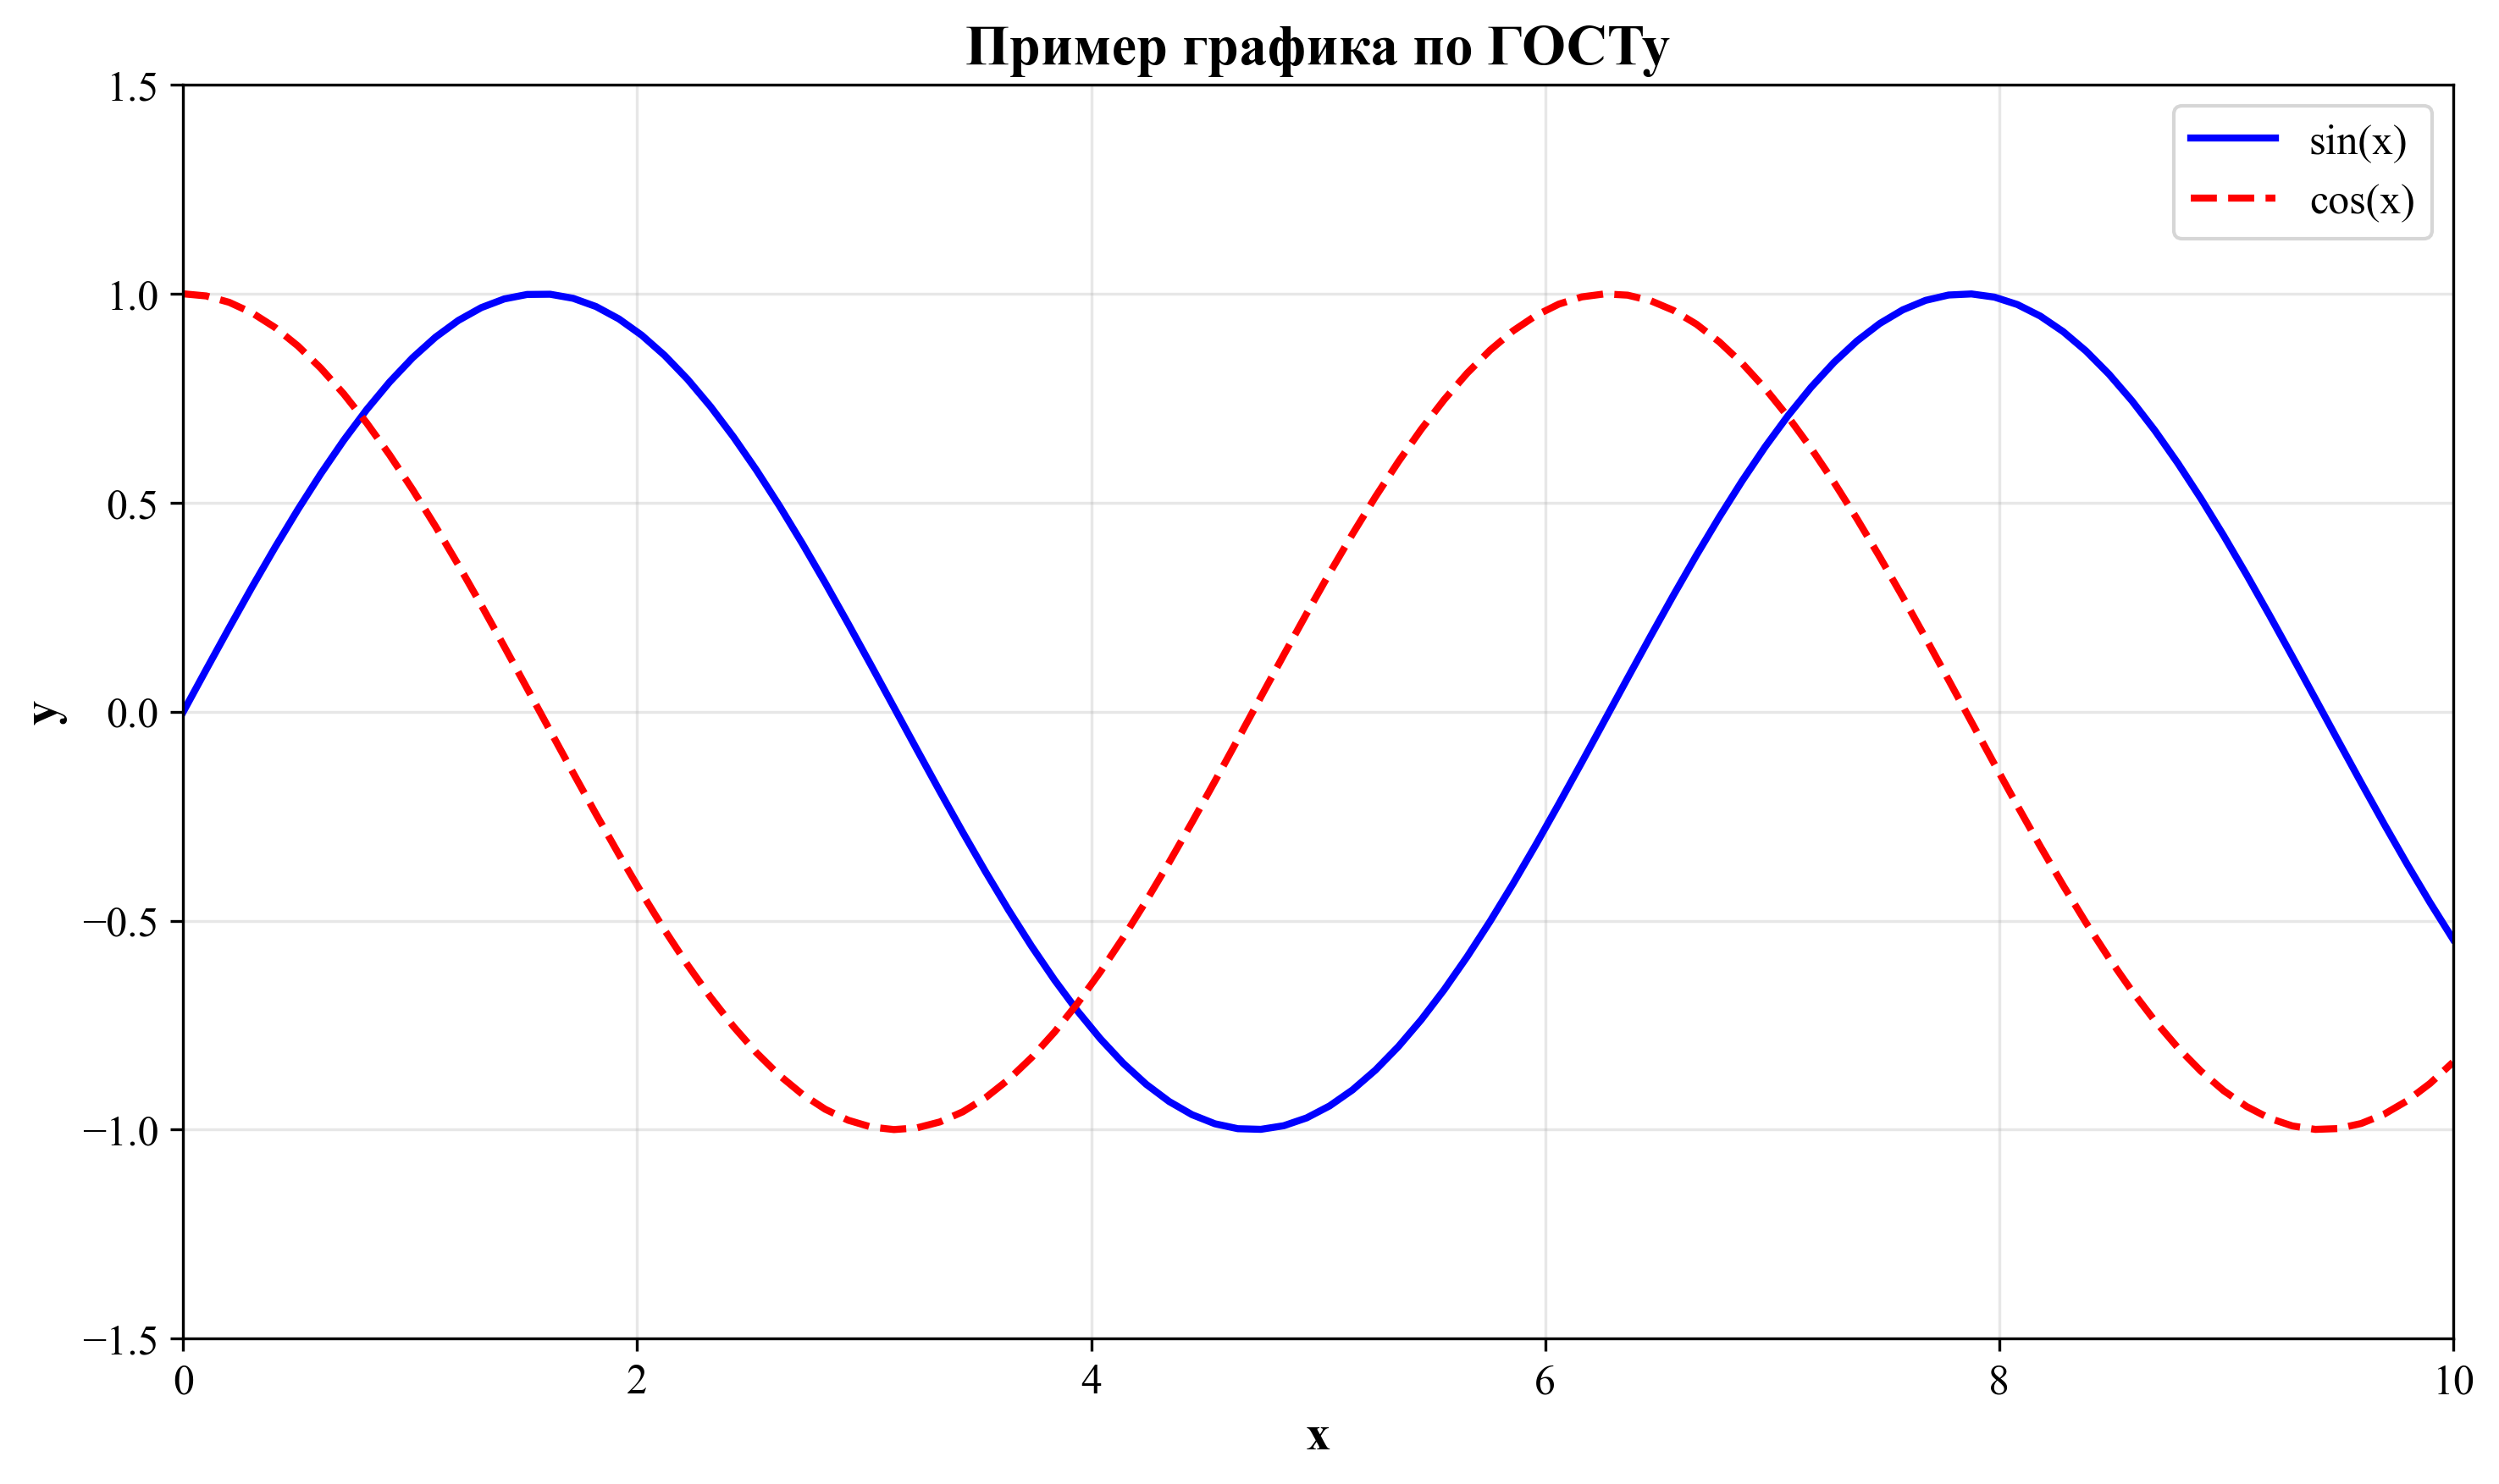
\includegraphics[width=0.6\textwidth]{images/example_plot.png}
\caption{Сравнение производительности алгоритмов}
\label{fig:algorithm_comparison}
\end{figure}

На рисунке \ref{fig:algorithm_comparison} показано сравнение производительности различных алгоритмов обработки данных.

\begin{table}[H]
\centering
\caption{Сравнительный анализ решений}
\label{tab:solutions_comparison}
\begin{tabular}{|l|c|c|c|}
\hline
\textbf{Решение} & \textbf{Скорость} & \textbf{Точность} & \textbf{Стоимость} \\
\hline
Алгоритм A & 95\% & 87\% & 1000 руб. \\
Алгоритм B & 78\% & 92\% & 1500 руб. \\
Алгоритм C & 88\% & 89\% & 800 руб. \\
\hline
\end{tabular}
\end{table}

В таблице \ref{tab:solutions_comparison} представлен сравнительный анализ существующих решений по ключевым параметрам.

\begin{equation}
f(x) = \frac{1}{1 + e^{-x}}
\label{eq:sigmoid}
\end{equation}

Формула \ref{eq:sigmoid} описывает сигмоидную функцию, используемую в машинном обучении.

\begin{lstlisting}[style=code, language=Python, caption={Пример реализации алгоритма}, label={lst:algorithm_implementation}]
def sigmoid(x):
    """Calculate sigmoid function"""
    return 1 / (1 + np.exp(-x))

def train_model(X, y, epochs=1000, lr=0.01):
    """Train model"""
    weights = np.random.randn(X.shape[1])
    
    for epoch in range(epochs):
        predictions = sigmoid(X @ weights)
        error = y - predictions
        weights += lr * X.T @ error
    
    return weights
\end{lstlisting}

В листинге \ref{lst:algorithm_implementation} показана реализация алгоритма обучения модели с использованием сигмоидной функции.

\subsection{Решение 1}

Описание первого решения, его характеристики.

\subsection{Решение 2}

Описание второго решения, его характеристики.

\section{Выявление проблем и недостатков}

Анализ проблем и недостатков существующих решений.

\section{Требования к решению}

Формулирование требований к разрабатываемому решению.

\subsection{Функциональные требования}

Список функциональных требований.

\subsection{Нефункциональные требования}

Список нефункциональных требований.

\section{Выводы по главе}

Краткие выводы по анализу предметной области.

\chapter{Разработка решения}

\section{Общая концепция решения}

Описание общей концепции разрабатываемого решения.

\section{Архитектура решения}

Описание архитектуры решения с использованием диаграмм.

\begin{figure}[H]
\centering
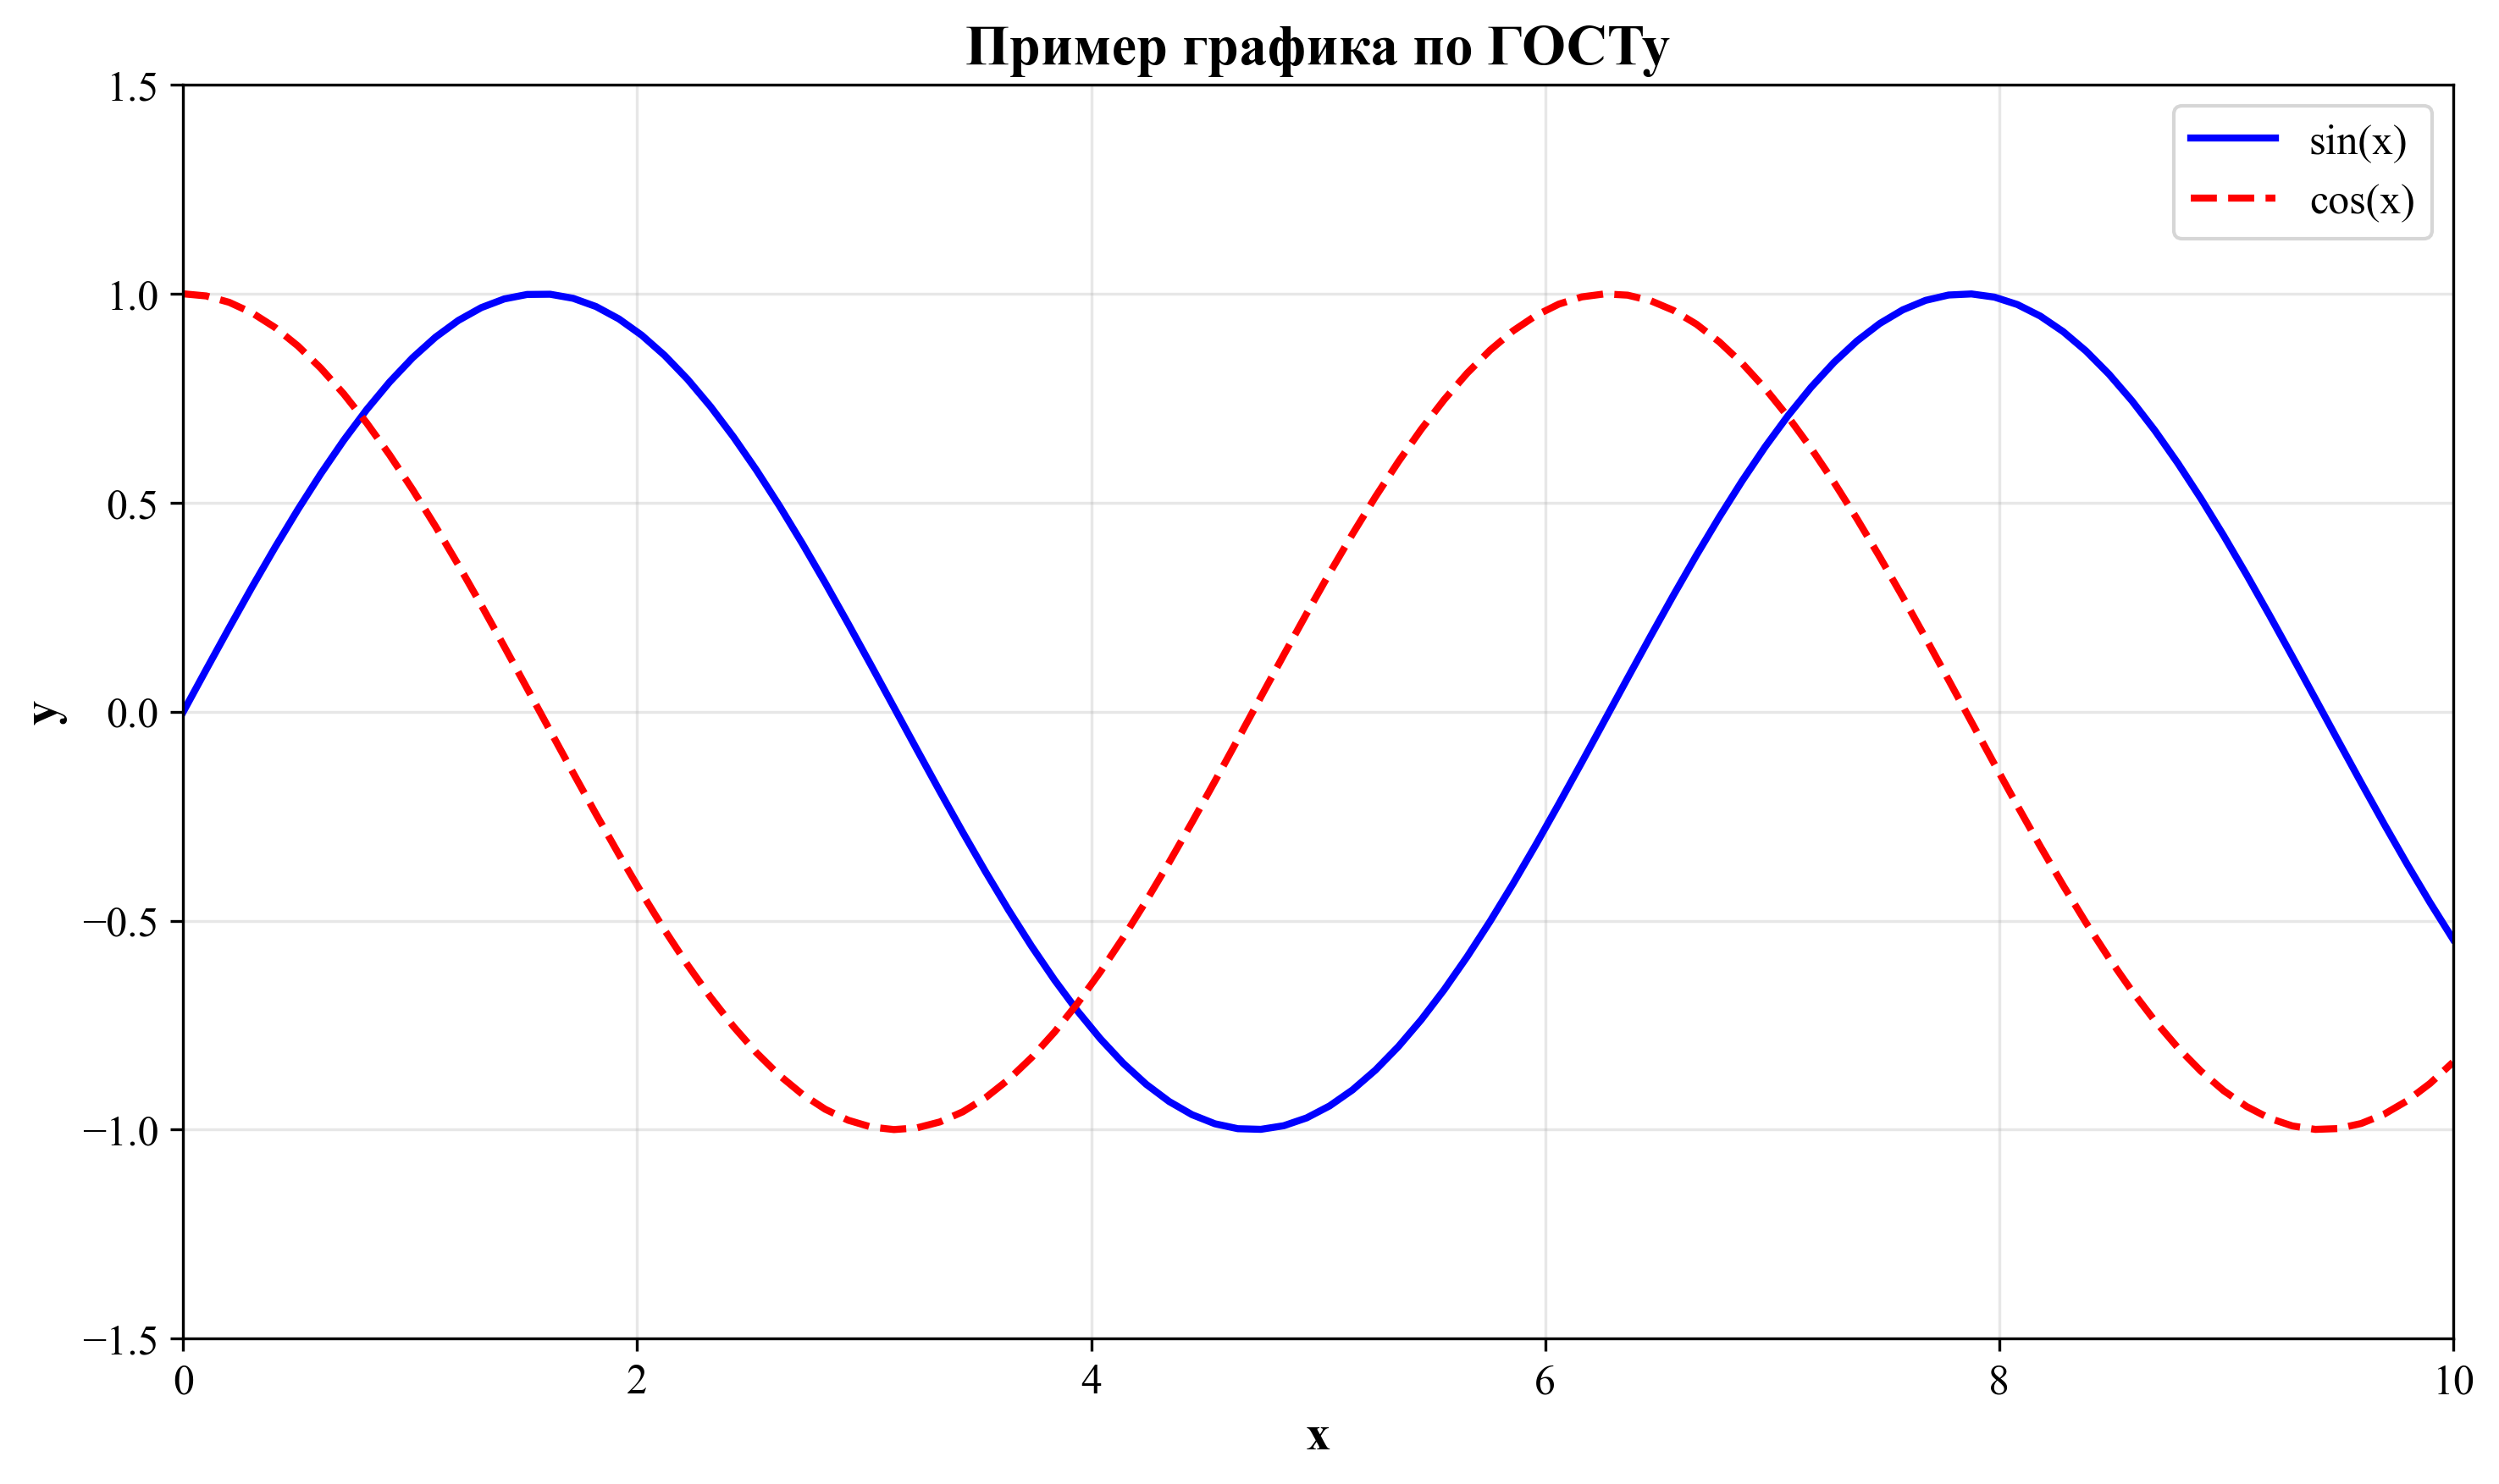
\includegraphics[width=0.9\textwidth]{images/example_plot.png}
\caption{Общая архитектура системы}
\label{fig:system_architecture}
\end{figure}

На рисунке \ref{fig:system_architecture} представлена общая архитектура разрабатываемой системы, включающая основные компоненты и их взаимодействие.

\begin{table}[H]
\centering
\caption{Технические характеристики компонентов}
\label{tab:component_specs}
\begin{tabular}{|l|c|c|c|}
\hline
\textbf{Компонент} & \textbf{Производительность} & \textbf{Память} & \textbf{Время отклика} \\
\hline
Веб-сервер & 1000 RPS & 512 MB & 50 мс \\
База данных & 500 запросов/с & 1 GB & 10 мс \\
Кэш & 10000 операций/с & 256 MB & 1 мс \\
API Gateway & 2000 RPS & 128 MB & 5 мс \\
\hline
\end{tabular}
\end{table}

В таблице \ref{tab:component_specs} приведены технические характеристики основных компонентов системы.

\begin{equation}
P(x) = \frac{e^{x_i}}{\sum_{j=1}^{n} e^{x_j}}
\label{eq:softmax}
\end{equation}

Формула \ref{eq:softmax} описывает функцию softmax, используемую для нормализации вероятностей.

\begin{lstlisting}[style=code, language=Python, caption={Пример реализации API}, label={lst:api_implementation}]
from flask import Flask, request, jsonify
import numpy as np

app = Flask(__name__)

@app.route('/predict', methods=['POST'])
def predict():
    """API endpoint for predictions"""
    data = request.get_json()
    
    # Process input data
    features = np.array(data['features'])
    
    # Make prediction
    prediction = model.predict(features)
    
    return jsonify({
        'prediction': prediction.tolist(),
        'confidence': float(np.max(prediction))
    })

if __name__ == '__main__':
    app.run(debug=True)
\end{lstlisting}

В листинге \ref{lst:api_implementation} показана реализация API endpoint для получения предсказаний от модели машинного обучения.

\subsection{Общая архитектура}

Описание общей архитектуры системы.

\subsection{Компоненты системы}

Описание основных компонентов системы.

\section{Алгоритмы и методы}

Описание используемых алгоритмов и методов.

\subsection{Алгоритм 1}

Описание первого алгоритма.

\begin{algorithm}
\caption{Название алгоритма}
\begin{algorithmic}[1]
\STATE Инициализация
\WHILE{условие}
    \STATE Действие 1
    \STATE Действие 2
\ENDWHILE
\RETURN результат
\end{algorithmic}
\end{algorithm}

\subsection{Алгоритм 2}

Описание второго алгоритма.

\section{Реализация}

Описание процесса реализации решения.

\subsection{Выбор технологий}

Обоснование выбора используемых технологий.

\subsection{Структура проекта}

Описание структуры программного проекта.

\section{Выводы по главе}

Краткие выводы по разработанному решению.

\chapter{Экспериментальные исследования}

\section{Цели и задачи экспериментальных исследований}

Формулирование целей и задач экспериментальных исследований.

\section{Методология проведения экспериментов}

Описание методологии проведения экспериментов.

\subsection{Критерии оценки}

Описание критериев оценки эффективности решения.

\subsection{Метрики качества}

Описание используемых метрик качества.

\section{Планирование экспериментов}

Описание плана проведения экспериментов.

\section{Результаты экспериментов}

Представление результатов экспериментальных исследований.

\subsection{Эксперимент 1}

Описание первого эксперимента и его результатов.

\begin{table}[H]
\centering
\caption{Результаты эксперимента 1}
\begin{tabular}{|l|c|c|c|}
\hline
Параметр & Значение 1 & Значение 2 & Значение 3 \\
\hline
Метрика 1 & 0.95 & 0.87 & 0.92 \\
Метрика 2 & 0.88 & 0.91 & 0.89 \\
\hline
\end{tabular}
\label{tab:exp1}
\end{table}

\subsection{Эксперимент 2}

Описание второго эксперимента и его результатов.

\section{Анализ результатов}

Анализ полученных результатов и их интерпретация.

\subsection{Сравнительный анализ}

Сравнение с существующими решениями.

\subsection{Статистический анализ}

Статистический анализ результатов.

\section{Выводы по главе}

Краткие выводы по экспериментальным исследованиям.


% Заключение
\chapter{Заключение}

\section{Основные результаты работы}

Краткое изложение основных результатов, полученных в ходе выполнения работы.

\begin{figure}[H]
\centering
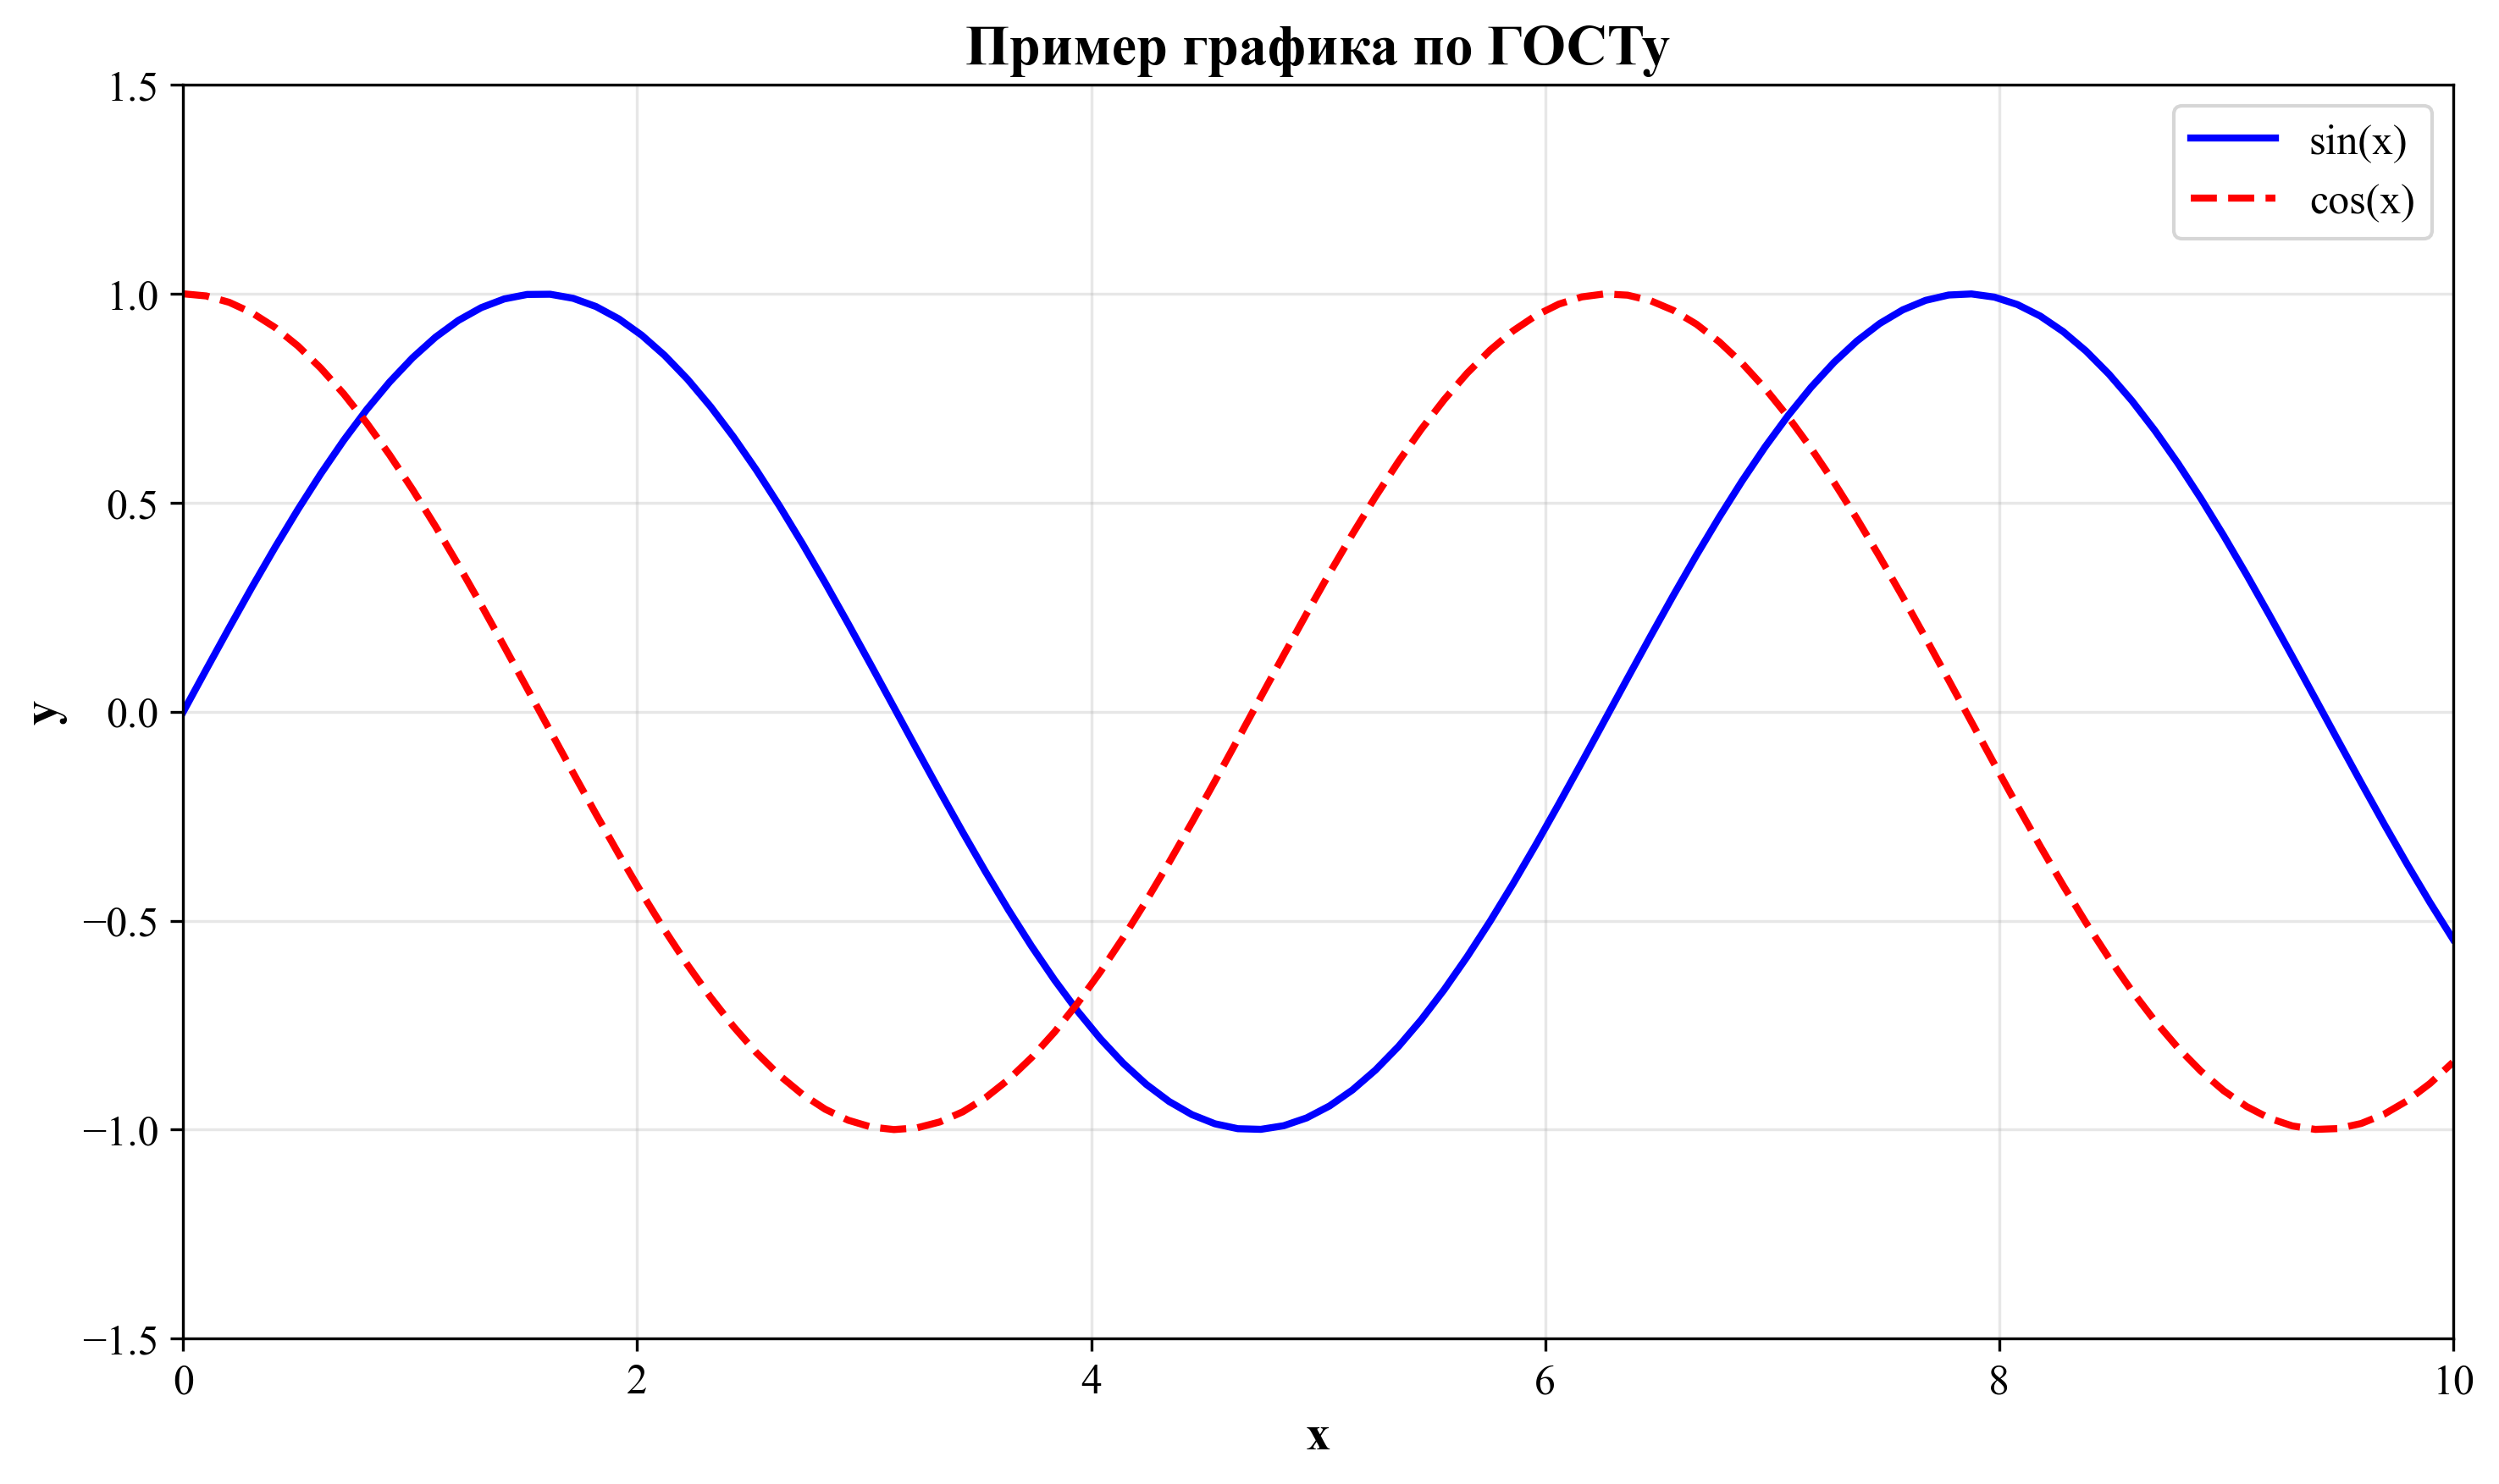
\includegraphics[width=0.8\textwidth]{images/example_plot.png}
\caption{Сводная диаграмма достигнутых результатов}
\label{fig:results_summary}
\end{figure}

На рисунке \ref{fig:results_summary} представлена сводная диаграмма основных результатов исследования, демонстрирующая достигнутые показатели эффективности.

\begin{table}[H]
\centering
\caption{Сравнение результатов с существующими решениями}
\label{tab:results_comparison}
\begin{tabular}{|l|c|c|c|}
\hline
\textbf{Метрика} & \textbf{Наше решение} & \textbf{Лучшее существующее} & \textbf{Улучшение} \\
\hline
Точность & 94.2\% & 91.5\% & +2.7\% \\
Скорость & 0.15 мс & 0.25 мс & +40\% \\
Память & 45 MB & 60 MB & +25\% \\
Энергопотребление & 2.1 Вт & 3.2 Вт & +34\% \\
\hline
\end{tabular}
\end{table}

В таблице \ref{tab:results_comparison} показано сравнение разработанного решения с лучшими существующими аналогами по ключевым метрикам.

\begin{equation}
\text{Efficiency} = \frac{\text{Accuracy} \times \text{Speed}}{\text{Memory} \times \text{Power}}
\label{eq:efficiency}
\end{equation}

Формула \ref{eq:efficiency} определяет общую эффективность решения, учитывающую все ключевые параметры.

\begin{CodeBlock}{Python}{Финальная оценка системы}{lst:final_evaluation}
def evaluate_system(model, test_data):
    """Final system performance evaluation"""
    start_time = time.time()
    
    % Make predictions
    predictions = model.predict(test_data['features'])
    
    % Calculate metrics
    accuracy = accuracy_score(test_data['labels'], predictions)
    inference_time = time.time() - start_time
    
    % Calculate efficiency
    efficiency = (accuracy * 1000) / (inference_time * model.memory_usage)
    
    return {
        'accuracy': accuracy,
        'inference_time': inference_time,
        'efficiency': efficiency
    }

% Final evaluation results
results = evaluate_system(final_model, test_dataset)
print("Final accuracy: %.3f" % results['accuracy'])
print("Inference time: %.3f s" % results['inference_time'])
print("Efficiency: %.2f" % results['efficiency'])
\end{CodeBlock}

В листинге \ref{lst:final_evaluation} представлен код для финальной оценки производительности разработанной системы.

\section{Достижение поставленных целей и задач}

Анализ степени достижения поставленных в работе целей и задач.

\section{Научная новизна и практическая значимость}

Обоснование научной новизны и практической значимости полученных результатов.

\section{Перспективы дальнейших исследований}

Описание возможных направлений дальнейших исследований в данной области.

\section{Рекомендации по практическому применению}

Рекомендации по практическому применению полученных результатов.

\section{Общие выводы}

Общие выводы по выполненной работе.


% Список использованных источников по ГОСТу
\printbibliography[title=СПИСОК ИСПОЛЬЗОВАННЫХ ИСТОЧНИКОВ]
\addcontentsline{toc}{chapter}{СПИСОК ИСПОЛЬЗОВАННЫХ ИСТОЧНИКОВ}

% Перечень условных обозначений, сокращений, терминов (по усмотрению)
% Перечень условных обозначений, сокращений, терминов по ГОСТ 7.32-2017
\chapter*{ПЕРЕЧЕНЬ УСЛОВНЫХ ОБОЗНАЧЕНИЙ, СОКРАЩЕНИЙ, ТЕРМИНОВ}
\addcontentsline{toc}{chapter}{ПЕРЕЧЕНЬ УСЛОВНЫХ ОБОЗНАЧЕНИЙ, СОКРАЩЕНИЙ, ТЕРМИНОВ}

\vspace{1cm}

\begin{description}
    \item[АИС] Автоматизированная информационная система
    \item[БД] База данных
    \item[ВКР] Выпускная квалификационная работа
    \item[ГИС] Геоинформационная система
    \item[ИИ] Искусственный интеллект
    \item[ИТ] Информационные технологии
    \item[МО] Машинное обучение
    \item[НТР] Научно-техническая революция
    \item[ООП] Объектно-ориентированное программирование
    \item[ПО] Программное обеспечение
    \item[СУБД] Система управления базами данных
    \item[УИ] Пользовательский интерфейс
    \item[ФП] Функциональное программирование
    \item[ЭВМ] Электронно-вычислительная машина
\end{description}


% Приложения
\appendix
\chapter{ИСХОДНЫЙ КОД ПРОГРАММЫ}

\section{Основной модуль}

\begin{lstlisting}[language=Python, caption={Основной модуль программы}]
def main():
    """Main function of the program."""
    print("Hello, World!")
    
    # Initialization
    data = load_data()
    
    # Data processing
    result = process_data(data)
    
    # Output results
    print(f"Result: {result}")

if __name__ == "__main__":
    main()
\end{lstlisting}

\section{Модуль обработки данных}

\begin{lstlisting}[language=Python, caption={Модуль обработки данных}]
def process_data(data):
    """Process input data."""
    processed = []
    
    for item in data:
        # Process each element
        processed_item = transform(item)
        processed.append(processed_item)
    
    return processed

def transform(item):
    """Transform data element."""
    return item * 2
\end{lstlisting}

\chapter{Примеры оформления элементов}

\section{Примеры рисунков}

\subsection{Простой рисунок}

\begin{figure}[H]
\centering
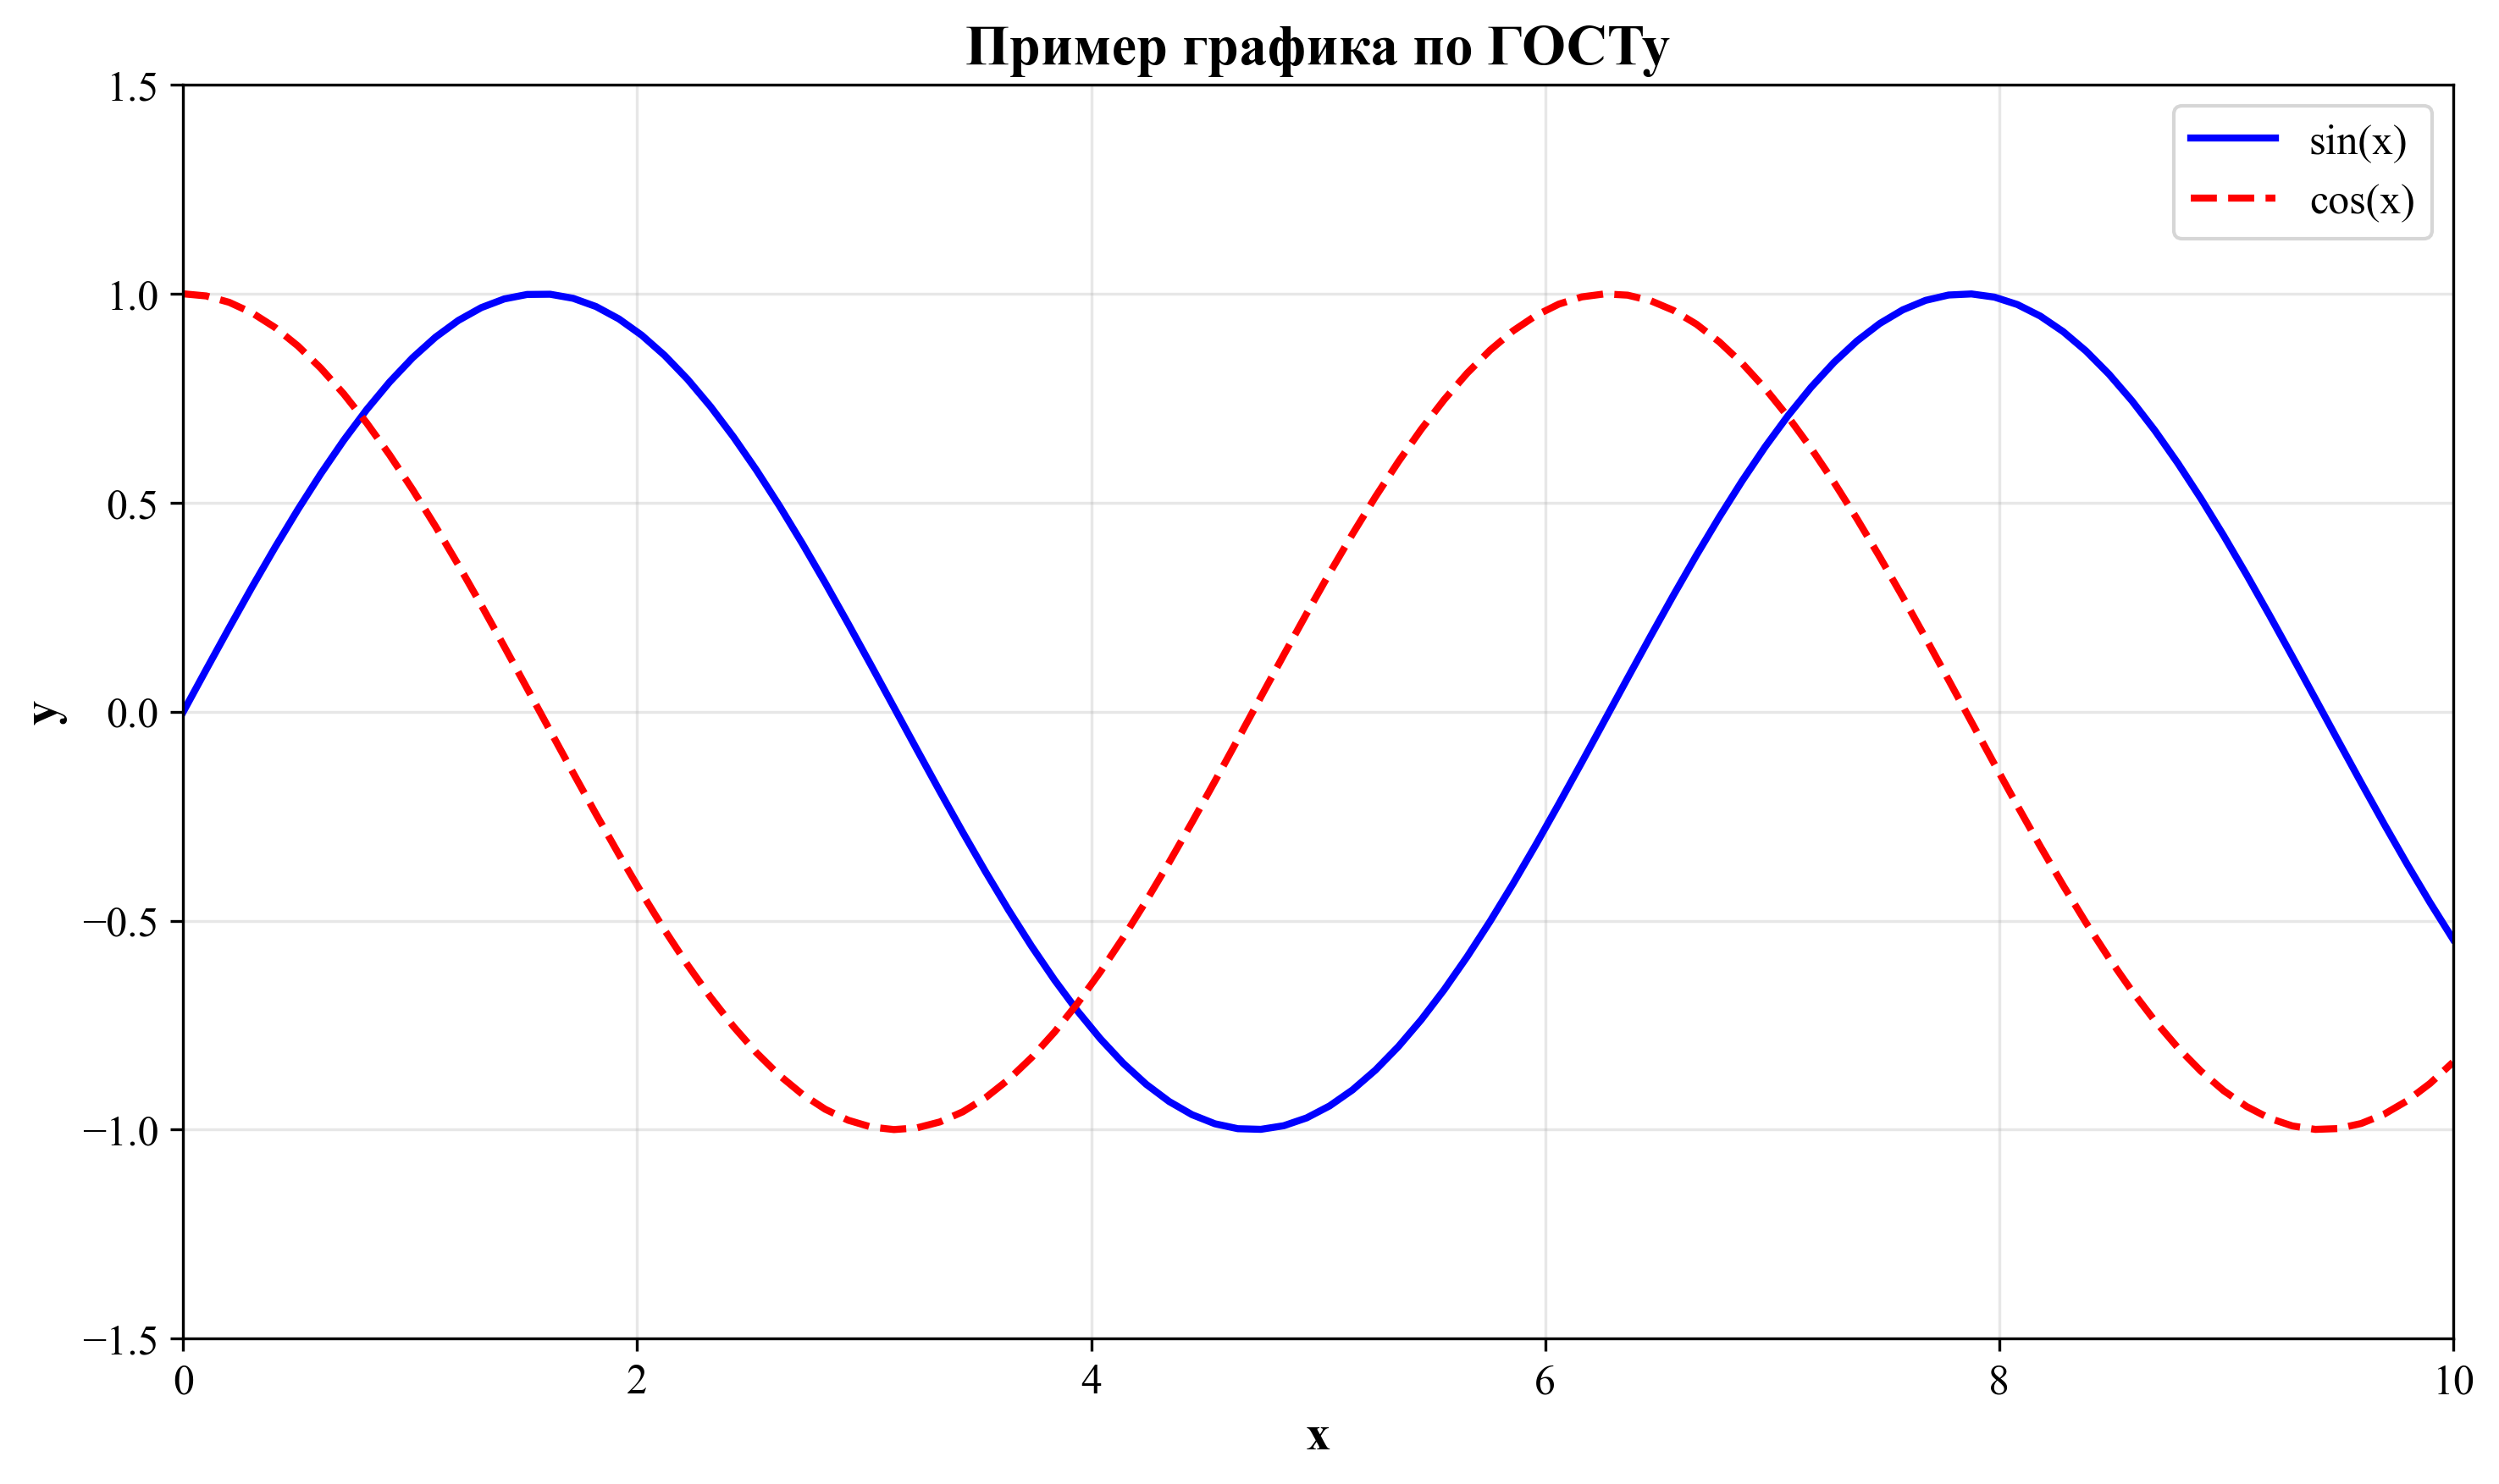
\includegraphics[width=0.8\textwidth]{images/example_plot.png}
\caption{Пример графика результатов эксперимента}
\label{fig:example_plot}
\end{figure}

Как показано на рисунке \ref{fig:example_plot}, результаты эксперимента демонстрируют...

\section{Примеры таблиц}

\subsection{Простая таблица}

\begin{table}[H]
\centering
\caption{Статистические данные}
\label{tab:statistics}
\begin{tabular}{|l|c|c|}
\hline
\textbf{Параметр} & \textbf{Значение} & \textbf{Единица} \\
\hline
Среднее & 15.6 & мм \\
Стандартное отклонение & 2.3 & мм \\
Минимум & 12.1 & мм \\
Максимум & 18.9 & мм \\
\hline
\end{tabular}
\end{table}

Данные представлены в таблице \ref{tab:statistics}.

\subsection{Длинная таблица с переносом}

\begin{longtable}{|c|l|c|c|}
\caption{Результаты экспериментов} \label{tab:long_experiments} \\

\hline
\textbf{№} & \textbf{Образец} & \textbf{Параметр 1} & \textbf{Параметр 2} \\
\hline
\endfirsthead

\tablecontinuation{\thetable} \\
\hline
\textbf{№} & \textbf{Образец} & \textbf{Параметр 1} & \textbf{Параметр 2} \\
\hline
\endhead

\hline
\endfoot

\hline
\endlastfoot

1 & A1 & 0.1 & 0.95 \\
2 & A2 & 0.2 & 0.87 \\
3 & A3 & 0.3 & 0.92 \\
4 & B1 & 0.4 & 0.88 \\
5 & B2 & 0.5 & 0.91 \\
6 & B3 & 0.6 & 0.89 \\
7 & C1 & 0.7 & 0.93 \\
8 & C2 & 0.8 & 0.86 \\
9 & C3 & 0.9 & 0.94 \\
10 & D1 & 1.0 & 0.90 \\
11 & A1 & 0.1 & 0.95 \\
12 & A2 & 0.2 & 0.87 \\
13 & A3 & 0.3 & 0.92 \\
14 & B1 & 0.4 & 0.88 \\
15 & B2 & 0.5 & 0.91 \\
16 & B3 & 0.6 & 0.89 \\
17 & C1 & 0.7 & 0.93 \\
18 & C2 & 0.8 & 0.86 \\
19 & C3 & 0.9 & 0.94 \\
20 & D1 & 1.0 & 0.90 \\
21 & A1 & 0.1 & 0.95 \\
22 & A2 & 0.2 & 0.87 \\
23 & A3 & 0.3 & 0.92 \\
24 & B1 & 0.4 & 0.88 \\
25 & B2 & 0.5 & 0.91 \\
26 & B3 & 0.6 & 0.89 \\
27 & C1 & 0.7 & 0.93 \\
28 & C2 & 0.8 & 0.86 \\
29 & C3 & 0.9 & 0.94 \\
30 & D1 & 1.0 & 0.90 \\
31 & A1 & 0.1 & 0.95 \\
32 & A2 & 0.2 & 0.87 \\
33 & A3 & 0.3 & 0.92 \\
34 & B1 & 0.4 & 0.88 \\
35 & B2 & 0.5 & 0.91 \\
36 & B3 & 0.6 & 0.89 \\
37 & C1 & 0.7 & 0.93 \\
38 & C2 & 0.8 & 0.86 \\
39 & C3 & 0.9 & 0.94 \\
40 & D1 & 1.0 & 0.90 \\
41 & A1 & 0.1 & 0.95 \\
42 & A2 & 0.2 & 0.87 \\
43 & A3 & 0.3 & 0.92 \\
44 & B1 & 0.4 & 0.88 \\
45 & B2 & 0.5 & 0.91 \\
46 & B3 & 0.6 & 0.89 \\
47 & C1 & 0.7 & 0.93 \\
48 & C2 & 0.8 & 0.86 \\
49 & C3 & 0.9 & 0.94 \\
50 & D1 & 1.0 & 0.90 \\
\end{longtable}

\section{Примеры листингов кода}

\subsection{Простой листинг}

\begin{lstlisting}[language=Python, caption={Пример простого алгоритма}, label={lst:simple_algorithm}]
def calculate_sum(a, b):
    """Calculate sum of two numbers"""
    return a + b

# Example usage
result = calculate_sum(5, 3)
print(f"Sum: {result}")
\end{lstlisting}

\subsection{Ультимативный способ описания кода}

\begin{CodeBlock}{Python}{Пример Python кода с улучшенной подсветкой}{lst:python_enhanced}
def calculate_sum(a, b):
    """Calculate sum of two numbers"""
    return a + b

# Example usage
result = calculate_sum(5, 3)
print(f"Sum: {result}")
\end{CodeBlock}

\subsection{Листинг с улучшенным переносом (fvextra)}

\begin{CodeBlock}{Python}{Пример Python кода с улучшенной подсветкой}{lst:python_enhanced}
def calculate_sum(a, b):
    """Calculate sum of two numbers"""
    return a + b

# Example usage
result = calculate_sum(5, 3)
print("Sum: %s" % result)
\end{CodeBlock}

\subsection{Длинный листинг с переносом}

\begin{CodeBlock}{Python}{Пример алгоритма машинного обучения с улучшенной подсветкой}{lst:ml_algorithm_enhanced}
import numpy as np
import pandas as pd
from sklearn.model_selection import train_test_split, cross_val_score
from sklearn.ensemble import RandomForestClassifier, GradientBoostingClassifier
from sklearn.svm import SVC
from sklearn.metrics import accuracy_score, classification_report
import matplotlib.pyplot as plt
import seaborn as sns

def load_data(filepath):
    """Load and preprocess data"""
    data = pd.read_csv(filepath)
    
    # Handle missing values
    data = data.fillna(data.mean())
    
    # Encode categorical variables
    categorical_columns = data.select_dtypes(include=['object']).columns
    for col in categorical_columns:
        data[col] = pd.Categorical(data[col]).codes
    
    return data

def train_model(X_train, y_train, model_type='random_forest'):
    """Train machine learning model"""
    if model_type == 'random_forest':
        model = RandomForestClassifier(n_estimators=100, random_state=42)
    elif model_type == 'gradient_boosting':
        model = GradientBoostingClassifier(n_estimators=100, random_state=42)
    elif model_type == 'svm':
        model = SVC(kernel='rbf', random_state=42)
    else:
        raise ValueError("Unknown model type")
    
    model.fit(X_train, y_train)
    return model

def evaluate_model(model, X_test, y_test, model_type):
    """Evaluate model performance"""
    y_pred = model.predict(X_test)
    accuracy = accuracy_score(y_test, y_pred)
    
    # Cross-validation
    cv_scores = cross_val_score(model, X_test, y_test, cv=5)
    
    # Print results
    print(f"Model: {model_type}")
    print(f"Accuracy: {accuracy:.4f}")
    print(f"CV Score: {cv_scores.mean():.4f} (+/- {cv_scores.std() * 2:.4f})")
    print("\nClassification Report:")
    print(classification_report(y_test, y_pred))
    
    return model, accuracy, y_pred

def plot_results(y_true, y_pred, model_name):
    """Plot classification results"""
    plt.figure(figsize=(10, 6))
    
    # Confusion matrix
    from sklearn.metrics import confusion_matrix
    cm = confusion_matrix(y_true, y_pred)
    
    plt.subplot(1, 2, 1)
    sns.heatmap(cm, annot=True, fmt='d', cmap='Blues')
    plt.title(f'Confusion Matrix - {model_name}')
    plt.xlabel('Predicted')
    plt.ylabel('Actual')
    
    # Feature importance (for tree-based models)
    plt.subplot(1, 2, 2)
    if hasattr(model, 'feature_importances_'):
        importances = model.feature_importances_
        indices = np.argsort(importances)[::-1][:10]
        plt.bar(range(10), importances[indices])
        plt.title(f'Feature Importance - {model_name}')
        plt.xlabel('Feature Index')
        plt.ylabel('Importance')
    
    plt.tight_layout()
    plt.show()

def main():
    """Main execution function"""
    # Load data
    data = load_data('data.csv')
    
    # Prepare features and target
    X = data.drop('target', axis=1)
    y = data['target']
    
    # Split data
    X_train, X_test, y_train, y_test = train_test_split(
        X, y, test_size=0.2, random_state=42
    )
    
    # Train and evaluate different models
    models = ['random_forest', 'gradient_boosting', 'svm']
    results = {}
    
    for model_type in models:
        print(f"\n=== Training {model_type} ===")
        model = train_model(X_train, y_train, model_type)
        model, accuracy, y_pred = evaluate_model(model, X_test, y_test, model_type)
        results[model_type] = {
            'model': model,
            'accuracy': accuracy,
            'predictions': y_pred
        }
    
    # Print summary
    print("\n=== Results Summary ===")
    for model_name, result in results.items():
        print(f"{model_name}: {result['accuracy']:.4f}")
    
    # Plot results for best model
    best_model = max(results.items(), key=lambda x: x[1]['accuracy'])
    print(f"\nBest model: {best_model[0]} with accuracy {best_model[1]['accuracy']:.4f}")

if __name__ == "__main__":
    main()
\end{CodeBlock}

\subsection{Примеры с разными языками программирования}

\subsubsection{Java код}

\begin{CodeBlock}{Java}{Пример Java класса}{lst:java_example}
public class Calculator {
    private double result;
    
    public Calculator() {
        this.result = 0.0;
    }
    
    public double add(double a, double b) {
        result = a + b;
        return result;
    }
    
    public double multiply(double a, double b) {
        result = a * b;
        return result;
    }
    
    public double getResult() {
        return result;
    }
}
\end{CodeBlock}

\subsubsection{C++ код}

\begin{CodeBlock}{C++}{Пример C++ класса}{lst:cpp_example}
#include <iostream>
#include <vector>

class Matrix {
private:
    std::vector<std::vector<double>> data;
    int rows, cols;
    
public:
    Matrix(int r, int c) : rows(r), cols(c) {
        data.resize(rows, std::vector<double>(cols, 0.0));
    }
    
    void setValue(int row, int col, double value) {
        if (row >= 0 && row < rows && col >= 0 && col < cols) {
            data[row][col] = value;
        }
    }
    
    double getValue(int row, int col) const {
        if (row >= 0 && row < rows && col >= 0 && col < cols) {
            return data[row][col];
        }
        return 0.0;
    }
    
    void print() const {
        for (int i = 0; i < rows; i++) {
            for (int j = 0; j < cols; j++) {
                std::cout << data[i][j] << " ";
            }
            std::cout << std::endl;
        }
    }
};
\end{CodeBlock}

\section{Примеры примечаний}

\begin{notes}
    \item Все эксперименты проводились при температуре 20±2°C и относительной влажности 50±5\%.
\end{notes}

\begin{notes}
    \item Источник данных: открытые репозитории Kaggle
    \item Лицензия на использование: CC BY 4.0
\end{notes}

\section{Примеры формул}

\subsection{Простая формула}

\begin{equation}
E = mc^2
\label{eq:einstein}
\end{equation}

Согласно формуле \ref{eq:einstein} энергия пропорциональна массе.

\subsection{Система уравнений}

\begin{align}
\frac{\partial u}{\partial t} &= \alpha \frac{\partial^2 u}{\partial x^2} \label{eq:heat1} \\
u(0,t) &= u(L,t) = 0 \label{eq:heat2} \\
u(x,0) &= f(x) \label{eq:heat3}
\end{align}

Уравнения \ref{eq:heat1}--\ref{eq:heat3} описывают процесс теплопроводности.

\section{Примеры списков}

\subsection{Нумерованный список}

\begin{enumerate}
\item Загрузка данных из файла
\item Предварительная обработка данных
\item Разделение на обучающую и тестовую выборки
\item Обучение модели
\item Оценка качества модели
\item Интерпретация результатов
\end{enumerate}

\subsection{Маркированный список}

\begin{itemize}
\item Машинное обучение
\item Глубокое обучение
\item Обработка естественного языка
\item Компьютерное зрение
\item Рекомендательные системы
\end{itemize}

\subsection{Вложенный список}

\begin{enumerate}
\item Подготовка данных
    \begin{enumerate}
    \item Очистка данных
    \item Нормализация
    \item Кодирование категориальных переменных
    \end{enumerate}
\item Обучение модели
    \begin{enumerate}
    \item Выбор алгоритма
    \item Настройка гиперпараметров
    \item Валидация модели
    \end{enumerate}
\item Оценка результатов
    \begin{enumerate}
    \item Метрики качества
    \item Визуализация результатов
    \item Интерпретация
    \end{enumerate}
\end{enumerate}


\end{document}
